
\section{Introdução}

\noindent \begin{minipage}[c]{0.6\textwidth}
  \vspace {1cm}
  \par A presente aula prática tem como fim a exploração do software Weka\ref{fig:logo_weka}, para a criação de uma rede neural Perceptron para interpretar corretamente os diferentes tipos de saídas do modelo.
  \par Para este fim é proposto o uso do software \href{https://www.cs.waikato.ac.nz/ml/index.html}{Weka}\ref{fig:logo_weka}, desenvolvido pela universidade do \href{https://www.waikato.ac.nz/}{Waikato} da Nova Zelândia, de acordo com \citeonline{Weka:2023}, o projeto possui quatro objetivos:
  \begin{asparaenum}
    \item tornar as técnicas de ML geralmente disponíveis;
    \item aplicá-los a problemas práticos importantes para a indústria da Nova Zelândia;
    \item desenvolver novos algoritmos de aprendizado de máquina e distribuí-los ao mundo;
    \item contribuir para um alicerce teórico para a área.
  \end{asparaenum}

\end{minipage}
\begin{minipage}[c]{0.4\textwidth}

  
\includegraphics[width=\textwidth]{figure/weka-logo.jpg}
  	\label{fig:logo_weka}
    \captionof{figure}{Weka, \cite{Weka:2023}}
    %\captionof*{figure}{Fonte: \citeonline{linux:2023}}
\end{minipage}



\section{Métodos}
\par Os métodos aplicados nesta aula prática foi seguido o roteiro da \href{https://github.com/OgliariNatan/neuralPerceptron/blob/main/Aula%20pr%C3%A1tica.pdf}{aula prática}, no roteiro da presente aula, foi deixado em aberto os passos para a instalação do software Weka. Em consulta rápida na internet encontrei um documento público denominado de \href{https://github.com/OgliariNatan/neuralPerceptron/blob/main/ML-09weka.pdf}{"Introdução ao Weka"}, da universidade federal do Paraná. do autor David Menotti. Segui as orientação e conclui a instalação do software como demonstra a figura \ref{fig:home_weka}.
\begin{figure}[h]
  \center
  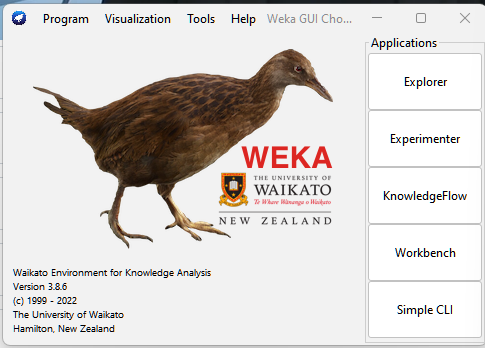
\includegraphics[scale=0.5]{figure/home_weka.png}
  \caption{Página inicial do Weka, O autor}\label{fig:home_weka}
\end{figure}
\par De acordo com o software, a versão instalada foi a \textbf{3.8.6}

\par Após a instalação do software e configurações adicionais, foi seguido as instruções do roteiro, ao qual solicitou que abrisse um arquivo chamado \textbf{"diabetes.arff"}, ao abrir o arquivo a software expressou as seguintes figuras \ref{fig:dados}.

\begin{figure}[H] %Figuras da aula pratica 1.1
  \center
  \subfigure[Dados simplificados.\label{fig:frist}]{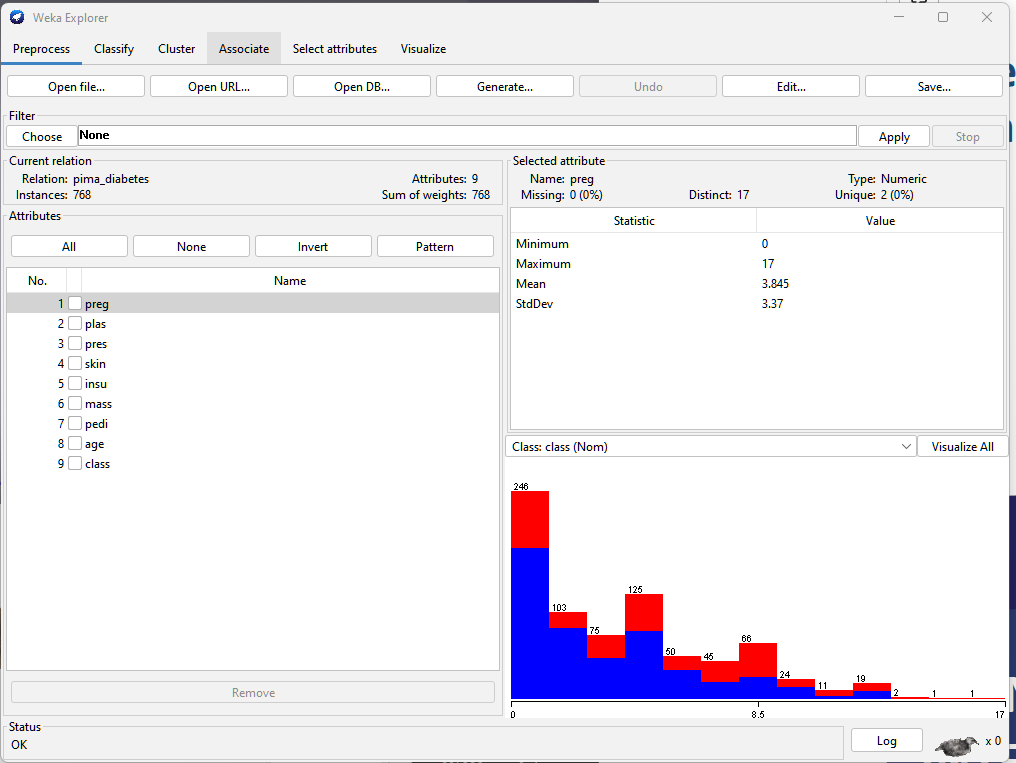
\includegraphics[scale=0.6]{figure/open_project.png}}
  \subfigure[Dados totais.\label{fig:75}]{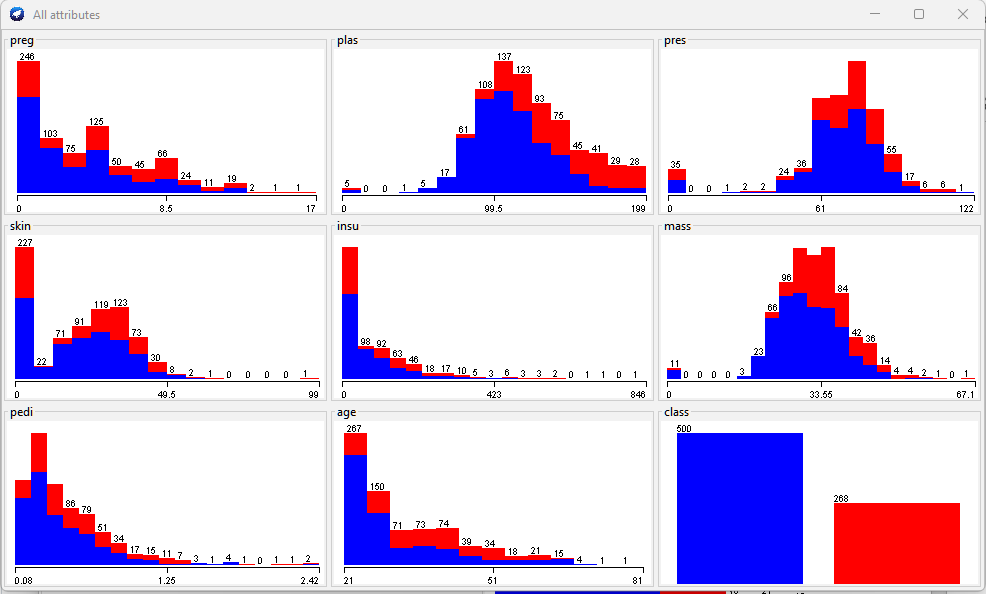
\includegraphics[scale=0.6]{figure/visualizeAll.png}}
  \caption{Dados Diabetes.arff, O autor}\label{fig:dados}
\end{figure}
\par Na sequência foi estabelecido a rede neural \textbf{perceptron} conforme figura \ref{fig:escolha}.

\begin{figure}[h]
  \center
  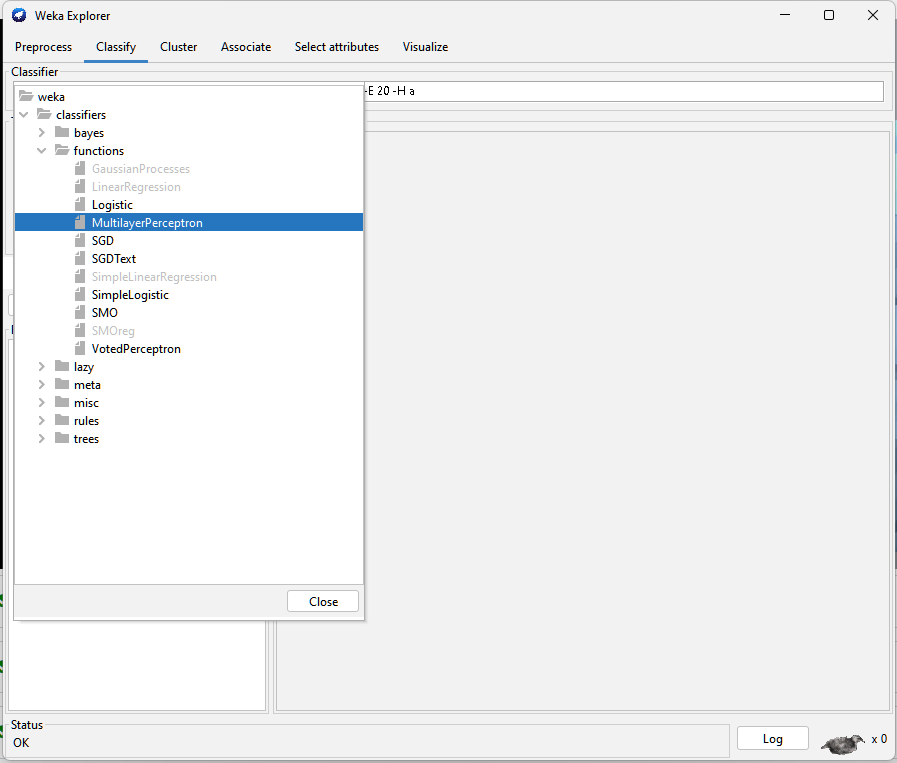
\includegraphics[scale=0.6]{figure/escolha_oerceptron.png}
  \caption{Escolha metodo Perceptron}\label{fig:escolha}
\end{figure}
%%%%%%%%%%%%%%%%%%%%%%%%%%%%%%%%%%%%%%%%%%%%%%%%%%%%%%%%%%

\section{Resultados}

\par De acordo com os resultados obtidos através da implementação da rede \textbf{Perceptron} figura \ref{fig:redeNeural} na fase de utilização, dispõe de oito entradas, uma camada interna com cinco possbilidades e duas saídas, sendo testes positivos \textit{testes\_positive} e testes negativos \textit{tested\_negative}. As figuras \ref{fig:frist} e \ref{fig:75}, são saídas da rede \textbf{Perceptron} para aula prática, a figura \ref{fig:75}, condiz ao condicionamento de que 75\% dos dados foram indicados para testes e o restante para treino do modelo da rede neural.

\begin{figure}[H] %Figuras da aula pratica 1.1
  \center
  \subfigure[Perceptron.\label{fig:frist}]{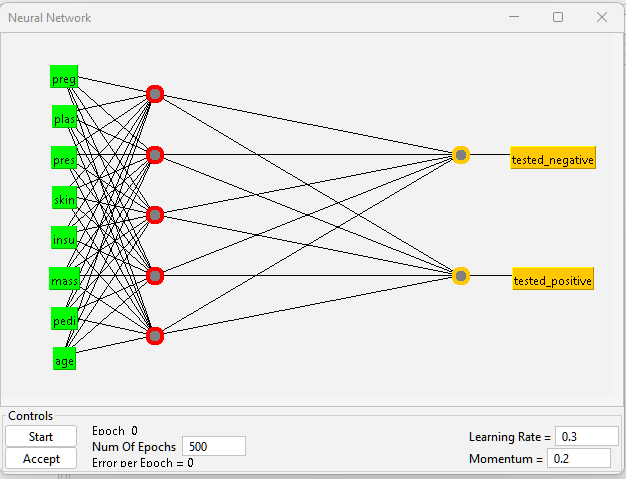
\includegraphics[scale=0.6]{figure/result.png}}

  \subfigure[Perceptron 75\%.\label{fig:75}]{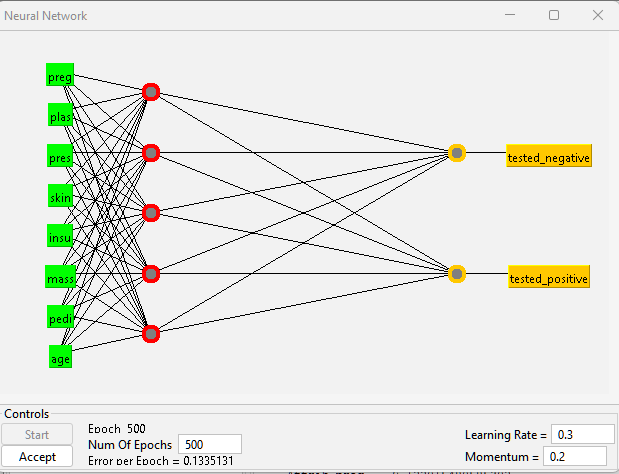
\includegraphics[scale=0.6]{figure/result_75p.png}}
  \caption{Rede neural Perceptron, O autor}\label{fig:redeNeural}
\end{figure}

\par No roteiro da aula prática foi solicitado que comparasse duas variavéis, sendo elas: \textit{Root mean squared error} "Raiz quadrada do erro médio" e \textit{Confusion Matrix} "Matriz de confusão" classificando em verdadeiro positivo, falso positivo, falso negativo e verdadeiro negativo. Para as duas análises como demonstra a figura \ref{fig:normal} e \ref{fig:75erro}.
\begin{figure}[H]
  \center
  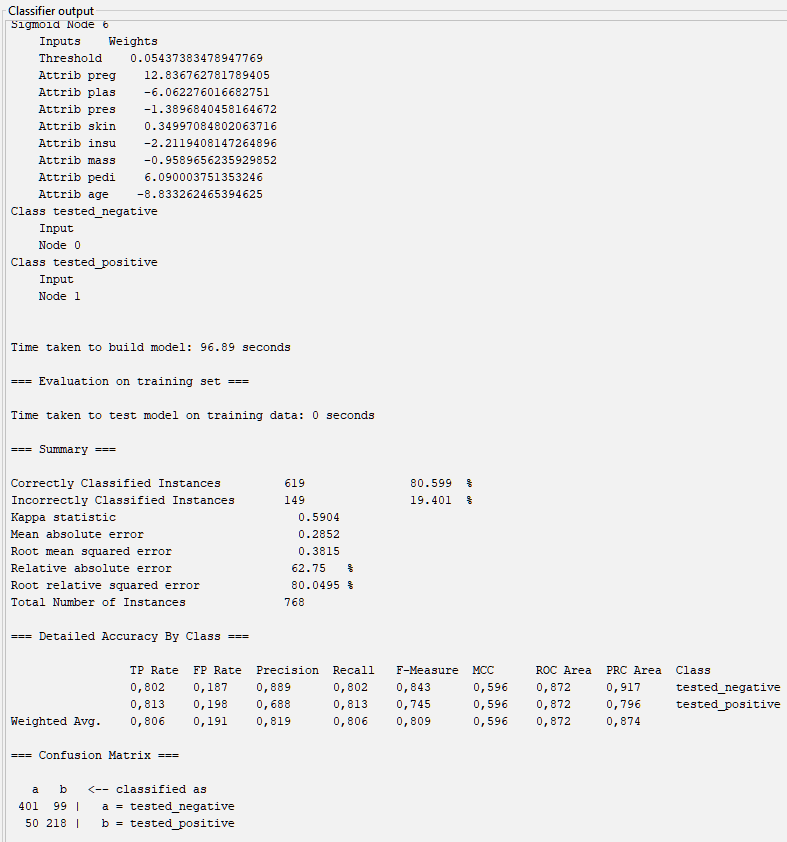
\includegraphics[scale=0.6]{figure/result_true3.png}
  \caption{log}\label{fig:normal}
\end{figure}

\begin{figure}[H]
  \center
  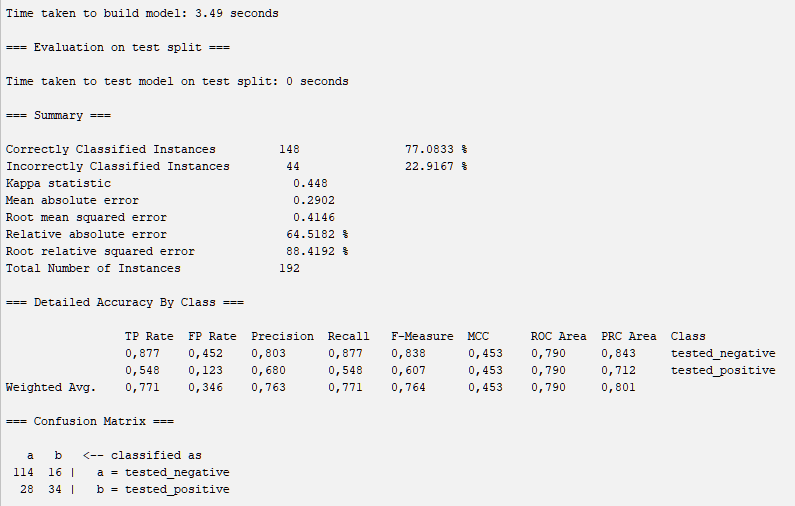
\includegraphics[scale=0.6]{figure/result_true_75p.png}
  \caption{log 75\%}\label{fig:75erro}
\end{figure}

\par A raiz quadrada do erro do primeiro teste foi de: 0.3815, e a matrix confusão é:
\begin{table}[h!]
\center
  \begin{tabular}{| c | c | c |}
  \hline
    a & b & Classificação\\
    \hline
    401 & 99 &  a = tested\_negative\\
    50 & 218 &  b = tested\_positive\\
    \hline
  %\caption{title}
  \end{tabular}
  \caption{Matrix confusão, O autor}
  \label{tab:normal}
\end{table}
\par A raiz quadrada do erro do segundo teste foi de: 0.4146
\begin{table}[h!]
\center
  \begin{tabular}{| c | c | c |}
  \hline
    a & b & Classificação\\
    \hline
    114 & 16 &  a = tested\_negative\\
    28 & 34 &  b = tested\_positive\\
    \hline
  %\caption{title}
  \end{tabular}
\caption{Matrix confusão 75\%, O autor}
\label{tab:75}
\end{table}
%%%%%%%%%%%%%%%%%%%%%%%%%%%%%%%%%%%%%%%%%%%%%%%%%%%%%%%%%%%%%%%%%%%%%%%%%%%%%%%%%%%%%%%
\section{Conclusões}
\par Observa-se que os dois teste com o treinamento da rede da figura \ref{fig:normal} e figura \ref{fig:75erro}, apresentam resultados levemente distintos, devido as quantidades de dados, sendo que a da figura \ref{fig:75erro} foi ordenado ao software weka que apenas 75\% dos dados para análise e 25\% para testes. Deta forma evedência a importancia do entendimento das redes neurais.
\par Da mesma forma as tabelas \ref{tab:normal} e \ref{tab:75}, demonstra a classificação da matriz confusão em testes positivos e teste negativos.



  %$X \xLongleftarrow[\text{NATAN}]{\text{OGLIARI}} Y $ %COM TEXTO
	% $\uparrow$ %Seta para Cima
	%$\overleftarrow{NATAN}$
